\documentclass{article}
\usepackage{amsthm,amsmath,amsfonts,lipsum}
\usepackage[T1]{fontenc}
\usepackage{beramono}
\usepackage{listings}
\usepackage{fontawesome5}
\usepackage{adjustbox}
\usepackage{mathabx}
\usepackage{thmtools}
\usepackage{import}
\usepackage{graphicx}
\usepackage{setspace}
\usepackage{geometry}
\usepackage{physics}
\usepackage{float}
\usepackage[english]{babel}
\usepackage{framed}
\usepackage[dvipsnames,x11names]{xcolor}
\usepackage{tcolorbox}
\usepackage{fancyhdr}
\usepackage{hyperref}
\usepackage{booktabs}
\usepackage{enumitem}
\usepackage{cancel}
\usepackage{background}
\usepackage{units}

% Configuring the background
\backgroundsetup{
  scale=1, % Optional, scale if needed
  color=black, % Optional, set the image color, can be omitted
  opacity=0.18, % Optional, adjust opacity for watermark effect
  angle=0,
  position=current page.center, % Center the image on the page
  contents={
\includegraphics[width=1.75\paperwidth, height=1.75\paperheight, keepaspectratio]{ninym_ralei_leaf (watermarked by AlexanderTheMango)}} % Keeps aspect ratio and scales to fill the page
}

% Colours
\definecolor{darkgreen}{rgb}{0.0, 0.5, 0.0}
\definecolor{Firebrick}{rgb}{0.698, 0.132, 0.203}
\definecolor{Crimson}{rgb}{0.862745, 0.078431, 0.235294} % Crimson color
\definecolor{lightred}{rgb}{1.0, 0.819608, 0.819608} % Light red for background
\definecolor{MediumPurple}{rgb}{0.576, 0.439, 0.859}
\definecolor{chocolate}{rgb}{0.82, 0.41, 0.12} % Chocolate color definition

% Define custom tcolorbox styles for notes
\tcbuselibrary{skins, breakable}
\newtcolorbox{definitionbox}{colframe=RoyalBlue, colback=blue!5!white, title=Definition}
\newtcolorbox{examplebox}{colframe=ForestGreen, colback=green!5!white, title=Example}
\newtcolorbox{notebox}{colframe=RedOrange, colback=orange!5!white, title=Note}
\newtcolorbox{theorembox}{colframe=RoyalPurple, colback=purple!5!white, title=Theorem}

\newtcolorbox{propositionbox}{colframe=Goldenrod, colback=yellow!10!white, title=Proposition}
\newtcolorbox{remarkbox}{colframe=MidnightBlue, colback=blue!10!white, title=Remark}
\newtcolorbox{corollarybox}{colframe=OliveGreen, colback=green!10!white, title=Corollary}
\newtcolorbox{warningbox}{colframe=Crimson, colback=lightred, title=Warning}
\newtcolorbox{proofbox}{colframe=Black, colback=gray!10!white, title=Proof}
\newtcolorbox{questionbox}{colframe=Teal, colback=teal!10!white, title=Question}
\newtcolorbox{tipbox}{colframe=Goldenrod, colback=yellow!10!white, title=Tip}
\newtcolorbox{exercisebox}{colframe=darkgreen, colback=green!5!white, title=Exercise}
\newtcolorbox{solutionbox}{colframe=DodgerBlue4, colback=blue!5!white, title=Solution}
\newtcolorbox{algorithmbox}{colframe=Navy, colback=blue!10!white, title=Algorithm}
\newtcolorbox{conceptbox}{colframe=chocolate, colback=brown!10!white, title=Concept}
\newtcolorbox{illustrationbox}{colframe=Firebrick, colback=red!10!white, title=Illustration}
\newtcolorbox{intuitionbox}{colframe=MediumPurple, colback=purple!10!white, title=Intuition}
\newtcolorbox{answerbox}{colframe=RoyalBlue, colback=blue!10!white, title=Answer}

% Geometry settings
\geometry{letterpaper, portrait, includeheadfoot=true, hmargin=1in, vmargin=1in}
\onehalfspacing

% Header and footer
\pagestyle{fancy}
\fancyhf{}
\lhead{MAT232 - Lecture Notes}
\rhead{\thepage}
\lfoot{University of Toronto Mississauga}
\rfoot{\today}

% Document starts
\begin{document}
\renewcommand{\familydefault}{\rmdefault}

\begin{titlepage}
    \null % This is a TeX command that does nothing but is necessary for vfill to work correctly
    \vfill
    \begin{center}
        {\fontsize{40}{48}\selectfont \bfseries MAT232 - Lecture 13}
        \vspace{20pt} \\
        {\LARGE after partial derivatives?} \\
        \vspace{20pt}
        \textbf{AlexanderTheMango}
        \vspace{8pt}
        \\ Prepared for February 24, 2025
    \end{center}
    \vfill
\end{titlepage}

\begin{titlepage}
    \null % Ensures proper alignment with vfill
    \vfill
    \begin{center}
        {\Huge \textbf{Definitions and Theorems}} \\[20pt]
        \rule{\textwidth}{0.5mm} \\[15pt]
        {\Large \textit{Straight from the textbook — lots of fluff this time, more than what we need!}} \\[15pt]
        \rule{\textwidth}{0.5mm} \\[15pt]
        \textbf{Quick recap before diving into the lecture.}
    \end{center}
    \vfill
\end{titlepage}


\section*{Preliminary Definitions and Theorems}

% Definition: Polar Coordinates
\begin{definitionbox}
\textbf{Polar Coordinates.}  
Each point in the Cartesian plane can be represented in polar coordinates as an ordered pair $(r, \theta)$, where $r$ is the radial coordinate (distance from the origin), and $\theta$ is the angular coordinate (angle measured from the positive $x$-axis).  
The correspondence between Cartesian coordinates $(x, y)$ and polar coordinates $(r, \theta)$ is given by:
\[
x = r\cos\theta, \quad y = r\sin\theta, \quad r^2 = x^2 + y^2, \quad \tan\theta = \frac{y}{x}.
\]
\end{definitionbox}

% Theorem: Converting Points
\begin{theorembox}
\textbf{Theorem 1.4. Converting Points Between Coordinate Systems.}  
Given a point $P$ in the plane with Cartesian coordinates $(x, y)$ and polar coordinates $(r, \theta)$, the following conversion formulas hold true:
\[
x = r\cos\theta, \quad y = r\sin\theta,
\]
\[
r^2 = x^2 + y^2, \quad \tan\theta = \frac{y}{x}.
\]
These formulas can be used to convert between Cartesian and polar coordinates.
\end{theorembox}

% Example: Converting Coordinates
\begin{examplebox}
\textbf{Example 1.10. Converting Between Rectangular and Polar Coordinates.}
\begin{enumerate}
    \item Convert $(1, 1)$ to polar coordinates:  
    Use $x = 1$ and $y = 1$. Then:
    \[
    r^2 = x^2 + y^2 = 1^2 + 1^2 = 2 \implies r = \sqrt{2}, \quad \tan\theta = \frac{y}{x} = \frac{1}{1} = 1 \implies \theta = \frac{\pi}{4}.
    \]
    Therefore, $(1, 1)$ can be represented as $(\sqrt{2}, \pi/4)$ in polar coordinates.
\end{enumerate}
\end{examplebox}

% Problem-Solving Strategy: Plotting a Curve
\begin{conceptbox}
\textbf{Problem-Solving Strategy: Plotting a Curve in Polar Coordinates.}
\begin{enumerate}
    \item Create a table with two columns: one for $\theta$ values and one for $r$ values.
    \item Calculate the corresponding $r$ values for each $\theta$.
    \item Plot each ordered pair $(r, \theta)$ on the polar coordinate axes.
    \item Connect the points and observe the resulting graph.
\end{enumerate}
\end{conceptbox}

% Example: Graphing in Polar Coordinates
\begin{examplebox}
\textbf{Example 1.12. Graphing a Function in Polar Coordinates.}
Graph the curve defined by $r = 4\sin\theta$.  
\begin{enumerate}
    \item Create a table of values for $\theta$ and calculate $r$:
    \[
    \begin{array}{c|c|c|c|c|c|c}
    \theta & 0 & \frac{\pi}{6} & \frac{\pi}{4} & \frac{\pi}{2} & \pi & 2\pi \\
    \hline
    r & 0 & 2 & \sqrt{2} & 4 & 0 & 0
    \end{array}
    \]
    \item Plot the points and connect them to form the curve. The result is a circle with radius $2$ centered at $(0, 2)$ in rectangular coordinates.
\end{enumerate}
\end{examplebox}

\begin{titlepage}
    \null % Ensures proper alignment with vfill
    \vfill
    \begin{center}
        {\Huge \textbf{Let’s Get Started}} \\[20pt]
        \rule{\textwidth}{0.5mm} \\[15pt]
        {\Large \textit{Time to dive into the lecture notes.}} \\[15pt]
        \rule{\textwidth}{0.5mm} \\[15pt]
        \textbf{Grab your pen or pencil, and let’s break this down step by step.}
    \end{center}
    \vfill
\end{titlepage}

\normalsize

\section*{Lecture Title}
\begin{notebox}
This template is designed for MAT232 lecture notes. Replace this content with your specific lecture details.
\end{notebox}

\section*{Recall 1st Year Calculus}
\begin{definitionbox}
A definite integral...
\end{definitionbox}
\begin{figure}[H]
    \centering
    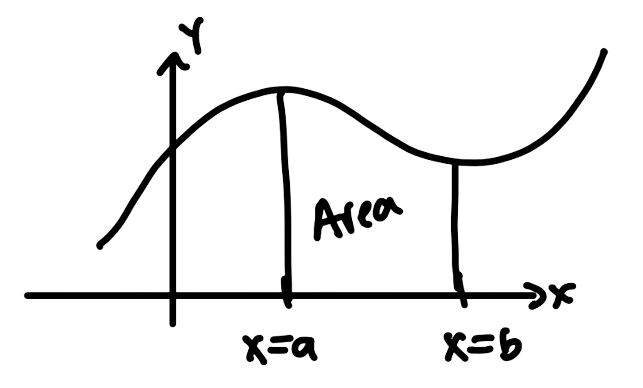
\includegraphics[width=0.6\textwidth]{1styearcalc.jpg}
    \caption{Sample image illustrating the concept.}
    \label{fig:sample_image}
\end{figure}

\section*{Section 1.2 (...cont'd): Now, in MAT232...}
\begin{definitionbox}
    \textbf{self-note: make this definition proper}
    A \textbf{parametric curve} has properties
    \[
        x = f(t), \quad y = g(t), \quad \alpha \leq t \leq \beta
    \]
    above the x-axis, and does not self-intersect.
    \textbf{self-note: show an image of self intersection and a cross to denote the ``NO!''}
    \[
        Area = \int_{x=a}^{x=b} f(x) dx = \int_{b}^{a} y(x) dx = \int_{c}^{d} x(y) dy
    \]
    Aside:
    \[
        Area = \int_{y=e}^{y=d} g(y) dy
    \]
    Also\dots
    \[
        Area = \int_{t=\alpha}^{t=\beta} g(t) f'(t) dt
    \]
    \[
        Area = \int_{t=\alpha}^{t=\beta} f(t) g'(t) dt
    \]
\end{definitionbox}

\section*{Examples}
\begin{examplebox}
\textbf{Example 1:} Find the area under the curve of the cycloid defined by the equations
\[ x = t - \sin(t), \quad y = 1 - \cos(t), \quad 0 \leq t \leq 2\pi. \]
\begin{itemize}
    \item \( x = f(t) = t - \sin(t) \) 
    \item \( x' = f'(t) = 1 - \cos(t) \) 
    \item \( y = g(t) = 1 - \cos(t) \)
\end{itemize}
Recall the generic formula to find the area:
\[
    Area = \int_{t=\alpha}^{t=\beta} g(t) f'(t) dt
\]
Applying \( f(t), g(t) \) from this question:
\begin{equation*}
    \begin{aligned}
        Area &= \int_{0}^{2\pi} [1 - \cos(t)][1 - \cos(t)] dt \\
        &= \int_{0}^{2\pi} [1 - 2\cos(t) + cos^2(t)] dt
    \end{aligned}
\end{equation*}
Recall the half-angles trigonometric identity:
\[
    \int_{}^{} \cos^2(x) dx = \int_{}^{} \frac{1 + cos(2x)}{2} dx
\]
\[
    \int_{}^{} \cos(x) dx = \sin(x) + c
\]
So\dots
\textbf{self-note: finish off the work below on the ellipsis}
\begin{equation*}
    \begin{aligned}
        Area &= \dots \\
        &= 3\pi
    \end{aligned}
\end{equation*}
\end{examplebox}


\section*{Homework Practice Question}
\begin{examplebox}
    Find the area under the curve defined by
    \[
        x = 3\cos(t) + \cos(3t), \quad y = 3\sin(t) - \sin(3t), \quad 0 \leq t \leq \pi.
    \]
    Hint: Recall that \( \sin^2(x) + \cos^2(x) = 1 \).
    Notice that...
    \[
        mathgoeshere
    \]
    \textbf{answer:} \( 3\pi \) 
\end{examplebox}

\section*{The Arc Length of a Parametric Curve}
\begin{theorembox}
\textbf{Theorem:} \textbf{self-note: grab the actual theorem from the textbook lol}

\begin{itemize}
    \item \( (x_1, y_1) \) and \( (x_2, y_2) \) are points
    \item \( \Delta x = x_1 - x_2 \), \( \Delta = \text{Delta} \) 
\end{itemize}
The distance between two points is denoted by \( D \) as follows:
\[
    D = \sqrt{(x_1 - x_2)^2 + (y_1 - y_2)^2}
\]
Substitute \( \Delta x \) and \( \Delta y \) as follows:
\[
    D = \sqrt{\Delta x^2 + \Delta y^2} 
\]
It follows that\dots
\[
    D = \sqrt{(\frac{\Delta x}{\Delta t})^2 + (\frac{\Delta y}{\Delta t})^2 } \Delta t
\]
Now, notice the similarity to Riemann sums from MAT136. As \( \Delta x \to 0 \):
\[
    L = \int_{t=\alpha}^{t=\beta} \sqrt{(\frac{dx}{dt})^2 + (\frac{dy}{dt})^2} dt 
\]
\textit{\( L \) is the (arc) length of a curve. This is confirmed to be included on term test 1, and will be on the formula sheet.}

\end{theorembox}

\begin{figure}[H]
    \centering
    
\includegraphics[width=0.6\textwidth]{sample_image1.jpg}
    \caption{Graphical representation of the theorem.}
    \label{fig:sample_image1}
\end{figure}

\section*{Example}
\begin{examplebox}
    Find the arc length of the curve defined by
    \[
        x = 3\cos(t), \quad y = 3\sin(t), \quad t \in [0, 2\pi] \text{.}
    \]
    The arc length is denoted by \( L \). Evaluate as follows:
    \begin{equation*}
        \begin{aligned}
            L &= \int_{0}^{2\pi} \sqrt{(-3\sin(t))^2 + (3\cos(t))^2} dt \\
            &= \textbf{self-note: finish this using the notes in the camera roll}
        \end{aligned}
    \end{equation*}
\end{examplebox}

\section*{Homework Practice Problem}
\begin{notebox}
    Find the arc length of the curve defined by
    \[
        x = 3t^2, \quad y = 2t^3, \quad 1 \leq t \leq 3 \text{.}
    \]
    \textbf{self-note: do the solution to this} \\
    \\
\end{notebox}

\section*{Section 1.3: Polar Coordinates}
\begin{definitionbox}
    \textbf{give the actual definition here from the textbook lol} \\
    \\
    Cartesian Coordniates:
    \begin{figure}[H]
        \centering
        
\includegraphics[width=0.6\textwidth]{sample_image1.jpg}
        \caption{Graphical representation of the theorem.}
        \label{fig:sample_image1}
    \end{figure}
    Polar Coordinates:
    \begin{figure}[H]
        \centering
        
\includegraphics[width=0.6\textwidth]{sample_image1.jpg}
        \caption{Graphical representation of the theorem.}
        \label{fig:sample_image1}
    \end{figure}
    How to work with \textbf{Polar Coordinates}
    \begin{enumerate}
        \item Start from the origin, and trace positively along the x-axis by the amount of the radius
        \item Imagine a line segment connecting from the origin to the resultant point, and rotate this line segment \( \theta \) degrees about the origin
        \item The destination of the resultant point is the point represented by the polar coordinate \( (r, \theta) \).
    \end{enumerate}
    Converting from \textbf{Cartesian Coordinates} to \textbf{Polar Coordinates}:
    \begin{enumerate}
        \item \textbf{self-note: see camera roll to fill this in with}
    \end{enumerate}
    Converting from \textbf{Cartesian Coordinates} to \textbf{Polar Coordinates}:
    \begin{enumerate}
        \item \textbf{self-note: see camera roll to fill this in with}
    \end{enumerate}
\end{definitionbox}

\section*{Additional Notes}
\begin{notebox}
Always check the domain of the parameter $t$ when solving problems involving parametric equations.
\end{notebox}

\section*{Further Visualization}
\begin{figure}[H]
    \centering
    
\includegraphics[width=0.6\textwidth]{sample_image2.jpg}
    \caption{Additional visualization for parametric curves.}
    \label{fig:sample_image2}
\end{figure}

\end{document}
